\section{Description}

The overall system has the objective of graduating individuals in a manner that
is at the same time democratic, stimulating, meritocratic and able to prepare 
those same individuals for a life in a society where computers will
play a major role.

In order to do that with a decreased cost, both financial and social, it is wise
to use the existing structure where it is possible to do so, so that factor is
embedded in the project as well.

\subsection{The relationship with knowledge}

The first step of the system would be the self preparation of a given student
through a process of interaction with the knowledge. But what knowledge? Well,
before the system is constructed it will be the job of the competent
authorities, both private and public, to digitalize the best available content
of the existing superior educational system. That could be done through the
video capturing of the federal universities classes, plus the digitalization of
all the non copyrighted material. 

That content should be placed in a free and open environment in the internet,
where it would be available to every citizen that would be interested in it.
This system would be described only superficially here, because ideally it would
leverage all the modern existing web development techniques in the ``web 2.0''.
Those techniques would serve to guide the students, to promote socialization in
the form of forums, tests, iterative games and so on, where the students would
play not only with the resources available on the system, but with each other
projects and exercises. That, as Papert puts it, places the fun on the learning
process:

\begin{quotation} 
    Part of the fun is sharing, posting graphics on the walls, modifying and
    experimenting with each other's work, and bringing the ``new'' products back to
    the original inventors. Although the work at the computer is usually private it
    increases the children's desire for interaction. These children want to get
    together with others engaged in similar activities because they have a lot to
    talk about. 
    \cite{education:papert_mindstorms}
\end{quotation}

This space would, of course, grow in richness with every user increasing the
opportunities and sharing it's own epistemological experiences, not only in some
particular subjects, which of course would take place, but of the medium itself,
smoothing the learning curve with each generation of users and producing a more
fitted social intelligence in the process, like Papert again makes clear:

\begin{quotation}
    As with writing, so with music-making, games of skill, complex graphics,
    whatever: The computer is not a culture unto itself but it can serve to
    advance very different cultural and philosophical outlooks.
    \cite{education:papert_mindstorms}
\end{quotation}

Of course, one does not expect the users would be the only responsibles for the
system. The hired professors of the competent authorities should be available
with enough consistency to increase the quality of the discussions and of the
official content of the system. 

One important aspect is that the form of the courses could be highly flexible,
which means that one could approach some subject from several points of view,
according to one's own pace and vocation. That would be a form of Piagetian
thinking, because although there would be goals, as the it will be discussed
later, the student is completely free to choose how and when to face those goals,
and if they would be faced at all. 

\subsection{The guarantee of quality}

A skeptical of the last scenario could, with quite a lot of reason, ask: ``But
what about the quality of those students, or should we just hand diplomas to
everyone who claims to be ready?''. Our society clearly must have a way to
assure itself of the quality of those who want to perform critical functions,
such as engineers, physicians and several other professions who deal with human
life in their craft.    

The way that was proposed so far concerned itself with the student acquiring and
holding the knowledge. But what about testing? To that we should turn to what
society usually turns to find credibility, specialized institutions and the
government, and those credible institutions could build a streamlined, on-demand 
certification scheme. More specifically in the Brazilian case, the very
structure of the vestibular system (which is highly effective and encompassing)
could be used to certificate students on general or specific points. Those
authorities would have control over the tests and what set of tests would
encompass a given course. 

For instance, to be fully graduated in medicine one should have to complete the
certifications of medicine 1 all the way through medicine 10, each sequentially
and with a minimum grade. To ask for a given test to be applied some person
would only have to provide some documentation and pay some fee to cover the
costs of using the system, and in the next round of testing the wanted test
would be available on some testing facility that is nearest to the requirer. The
testing procedure per se would be audited by payed officers. The system would
indeed be the same as a normal vestibular.


\subsection{The needed physical step}

The model so far would be incomplete on our day and age, mostly because of the
limitations of the digital distribution model. That will probably change if we
follow Kurzweil ideas:

\begin{quotation}
    Because of current bandwidth limitations and the lack of effective
    three-dimensional displays, the virtual environment provided today through
    routine Web access does not yet fully compete with ``being there'', but that
    will change. In the early part of the second decade of this century
    visual-auditory virtual- reality environments will be full immersion, very
    high resolution, and very convincing. Most colleges will follow MIT's lead,
    and students will increasingly attend classes virtually. Virtual
    environments will provide high-quality virtual laboratories where
    experiments can be conducted in chemistry, nuclear physics, or any other
    scientific field. Students will be able to interact with a virtual Thomas
    Jefferson or Thomas Edison or even to \textit{become} a virtual Thomas
    Jefferson. Classes will be available for all grade levels in many languages.
    The devices needed to enter these high-quality, high-resolution virtual
    classrooms will be ubiquitous and affordable even in third world countries.
    Students at any age, from toddlers to adults, will be able to access the
    best education in the world at any time and from any place.
    \cite{futurism:kurzweil_singularity_is_near} 
\end{quotation}

But what could be done today to reproduce the physical training and
socialization required for the formation of a fully fledged professional or
researcher? That today would still need a physical gathering place. 

The steps explained earlier would provide that space, by freeing up the existing
classrooms that before were dedicated to teaching repeatedly stuff. Not only the
classrooms would be liberated, but the professors would be alleviated of most of
the burden of direct teaching the horde of new students that would arrive each
semester.   

If both professors and classrooms would have more capability, so workshops could
be created based on demand, and labs could use students with some
qualifications or characteristics for assistants. There would be a very lively
interplay between the institutions and those who wanted to partake on those
activities, and that process would be guided much by the individual, choosing
when and how to approach the institution. 

Those labs and workshops could, if certified by the authorities, also certify
students who are active on them, so there would be an extra motivation for
students to build their own projects, in a very constructionist way.

\clearpage

\subsection{Overview}

\begin{figure}[htb]
   \centering
   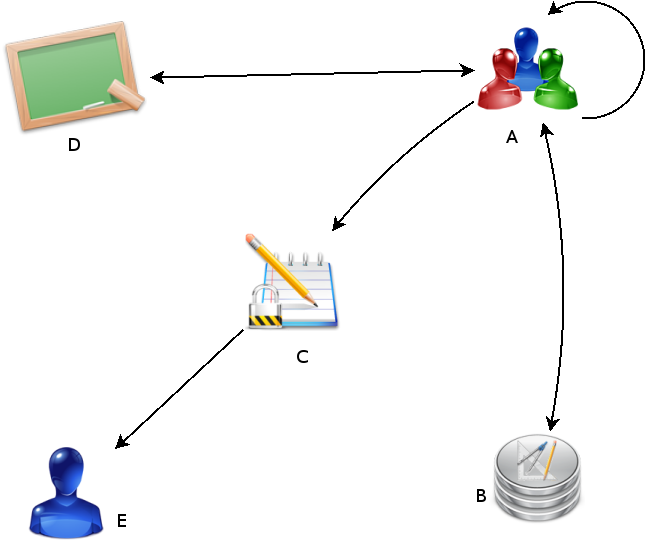
\includegraphics[width=1\columnwidth]{images/diagram.png}
   \caption{Overview diagram}
   \label{fig:overview_diagram}
\end{figure}


\begin{description}
    \item[A] The population interested in the system, the candidates.
    \item[B] The knowledge made available by the institutions.
    \item[C] The certification procedure.
    \item[D] The labs with a physical location, operated by faculty, mentors and the
    certificated students.
    \item[E] A graduated student.
\end{description}

